
\chapter{評価}
\label{sec:eval}
本章では,提案手法の評価を行う.\refsec{eval_env}で評価環境について説明し,\refsec{eval_segIQ}で提案手法によるタグ比較回数と性能低下の評価を行う.\refsec{eval_subseg}でサブ・セグメントに関する評価を説明した後,\refsec{eval_threshold}で SWITCH 方式のパラメータに関する評価を行い,\refsec{eval_ipc_comp}でセグメント数に関する評価について説明する.

\section{評価環境}
\label{sec:eval_env}
評価環境について説明する.性能やタグ比較回数を評価するために,SimpleScalar v.3.0a をベースに作成したシュミレータを使用した.評価で仮定したプロセッサ構成を\tab{base_config}に示す.

提案手法の SWITCH 方式に関するパラメータを,\tab{switch_config}に示す.これらのパラメータは,\refsec{eval_threshold} で説明する評価に基づいて決定した最適なパラメータである.

測定ベンチマークには,SPEC CPU 2017 ベンチマークのうち,int 系 9 本と fp 系 9 本の計 18 本を使用した.プログラムの入力には ref データ・セットを用いた.ベンチマークの測定区間は,プログラムの先頭から 16B 命令をスキップした後の 100M 命令である.

\begin{table}[htb]
  \caption{プロセッサの基本構成}
  \footnotesize
  \center
    \begin{tabular}{l|l} \hline \hline
     Pipeline width & 8 instructions wide for each of \\
     & fetch,decode,issue,and commit \\
     Reorder buffer & 300 entries \\
     IQ & 128 entries \\
     Load/Store queue & 128 entries \\
     Physical registers & 300(int) + 300(fp) \\
     Branch prediction & 16KB Perceptron predictor~\cite{Jimenez2001} \\
     & 2K-set 4-way BTB \\
     & 10-cycle misprediction penalty \\
     Function unit & 4 iALU,2 iMULT,\\
     &  3 FPU,2 LSU \\
     L1 D-cache & 32KB,8-way,64B line \\
      & 2-cycle hit latency \\
     L1 I-cache & 32KB,8-way,64B line \\
      &  2-cycle hit latency \\
     L2 cache & 2MB,16-way,64B line \\
      & 12-cycle hit latency \\  
     Main memory & 300-cycle latency \\
     & 8B/cycle bandwidth \\ 
     Prefetch & stream-based,32-stream tracked, \\ 
     & 16-line distance,2-line degree,\\
     & prefetch to L2 cache \\ \hline
  \end{tabular}
  \label{tab:base_config}
\end{table}

\begin{table}[tb]
  \caption{提案手法の SWITCH 方式に関するパラメータ構成}
  \footnotesize
  \center
    \begin{tabular}{l|l} \hline \hline
    切り替えインターバル & 10K instructions \\
    IPC しきい値 & 3.5 \\
    LLC MPKI しきい値 & 2.0 \\ \hline 
  \end{tabular}
  \label{tab:switch_config}
\end{table}

\subsubsection{ベンチマークの分類}
提案手法は,プログラムの ILP や MLP に着目した制御を行う.そこで,SPEC CPU 2017 ベンチマークを ILP が高いベンチマーク,MLP が高いベンチマーク,いずれも低いベンチマークの 3 種類に分類する.ここて,ILP 及びMLP が高いベンチマークとは,次の条件を満たすベンチマークである.
\begin{itemize}
  \item high ILP:IPCが 3.5以上のベンチマーク
  \item high MLP:LLC MPKI が2 以上のベンチマーク
\end{itemize}

分類結果を\tab{classification}に示す.また,以降に示す図において,ILP(青色) 及びMLP(赤色)の表記は,ILP もしくは MLP が高いベンチマークであることを表す.
\begin{table}[htb]
  \caption{ベンチマークの分類}
  \footnotesize
  \center
    \begin{tabular}{c|l} \hline \hline
    high ILP & xz,bwaves,cactuBSSN,cam4,\\
             & imagick,pop2,roms\\ \hline
    high MLP &  omnetpp,xalancbmk,lbm\\ \hline
    low ILP and low MLP & exchange2,leela,deepsjeng,mcf\\
                        & perlbench,x264,fotonik3d,nab \\ \hline
  \end{tabular}
  \label{tab:classification}
\end{table}

\subsubsection{評価モデル}
評価モデルは以下の 4 種類である.
\begin{itemize}
  \item BASE:セグメント化しない通常の IQ を使用するモデル
  \item AGGRESSIVE:提案手法において常に AGGRESSIVE モードで実行するモデル
  \item CONSERVATIVE:提案手法において常に CONSERVATIVE モードで実行するモデル
  \item SWITCH:提案手法の SWITCH 方式を使用するモデル 
\end{itemize}

\subsubsection{タグ比較回数の測定}
提案手法によるタグ比較回数の削減を評価するために,シミュレータでタグ比較の回数を測定した.ここで,タグ比較の回数とは,\textbf{ウェイクアップ時にレディでないオペランドの比較において,タグが一致しなかった数}とする.これは,タグ比較に関して以下のような仮定をおいているためである.

\begin{itemize}
  \item すでにレディなオペランドの比較器は動作しないとする.比較器のプリチャージを抑制することにより,容易に停止させることができるからである.
  \item デスティネーション・タグは,最大で発行幅分送られてくるが,送られてこなかったデスティネーション・タグのタグ線につながっている比較器は動作しないとする.これは,比較器のプリチャージ期間にタグ線を $L$ にするが,デスティネーション・タグが送られてこなければ,$L$ のままとすることは容易であるからである.
  \item タグが一致した比較器は,プリチャージされた電荷がディスチャージされないので,電力を消費しない.
\end{itemize}

\begin{figure}[htb]
  \centering
  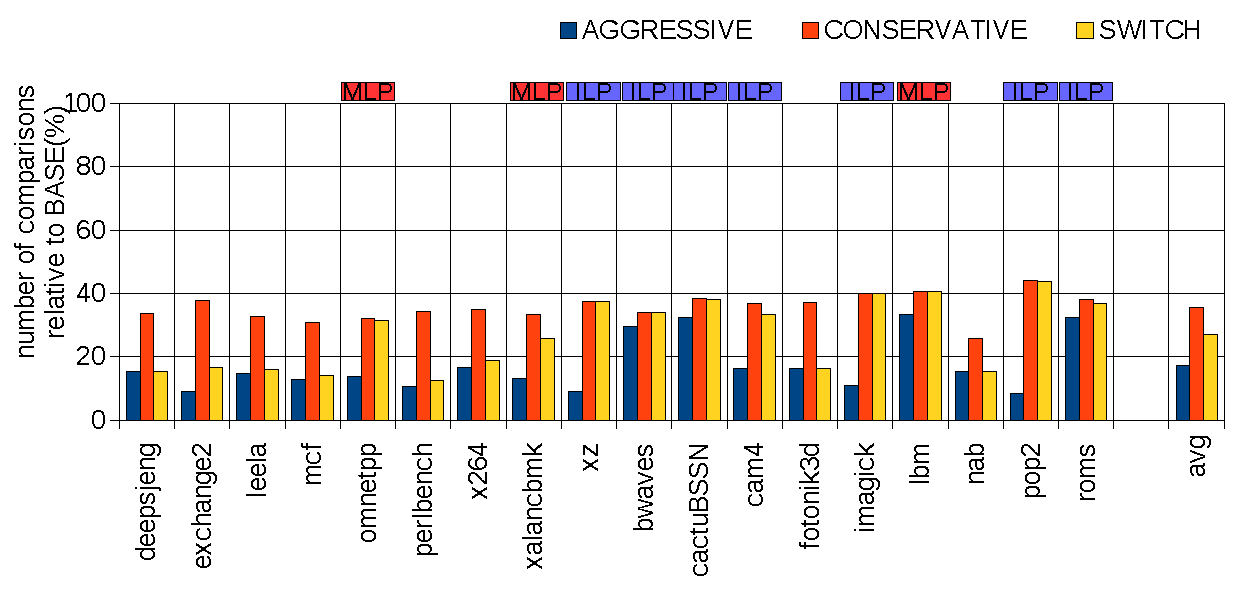
\includegraphics[keepaspectratio, scale=.8]{comp_16_1}
  \caption{提案手法によるタグ比較回数(16,1)}
  \label{fig:comp_16_1}
\end{figure}
\begin{figure}[htb]
  \centering
  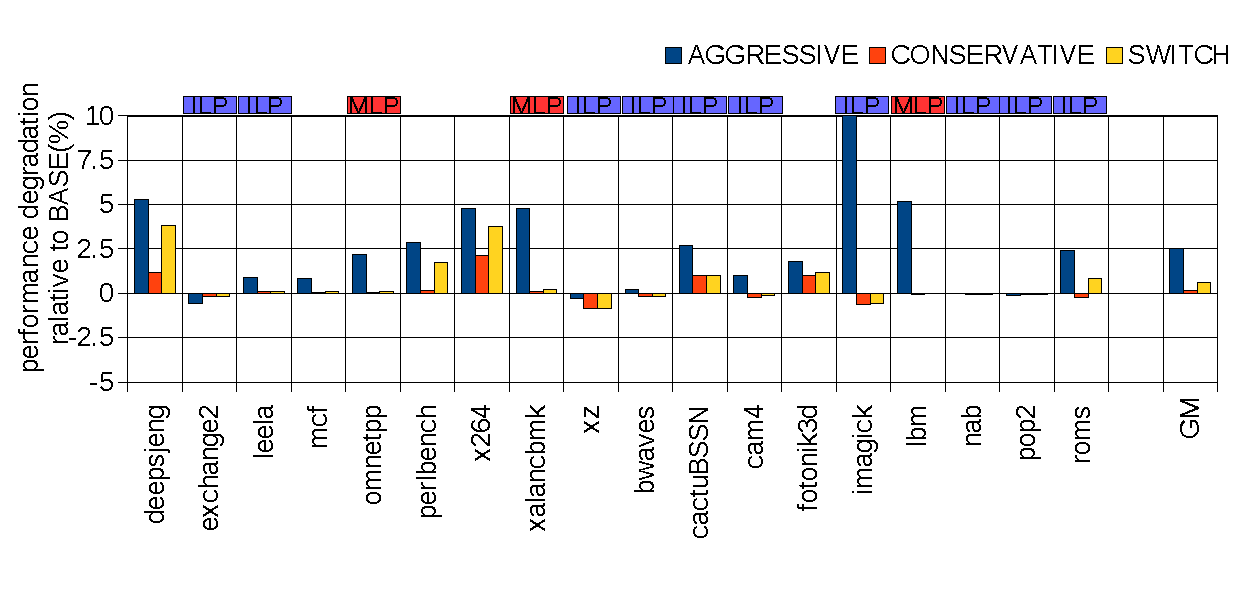
\includegraphics[keepaspectratio, scale=.8]{ipc_16_1}
  \caption{提案手法による性能低下(16,1)}
  \label{fig:ipc_16_1}
\end{figure}
\begin{figure}[htb]
  \centering
  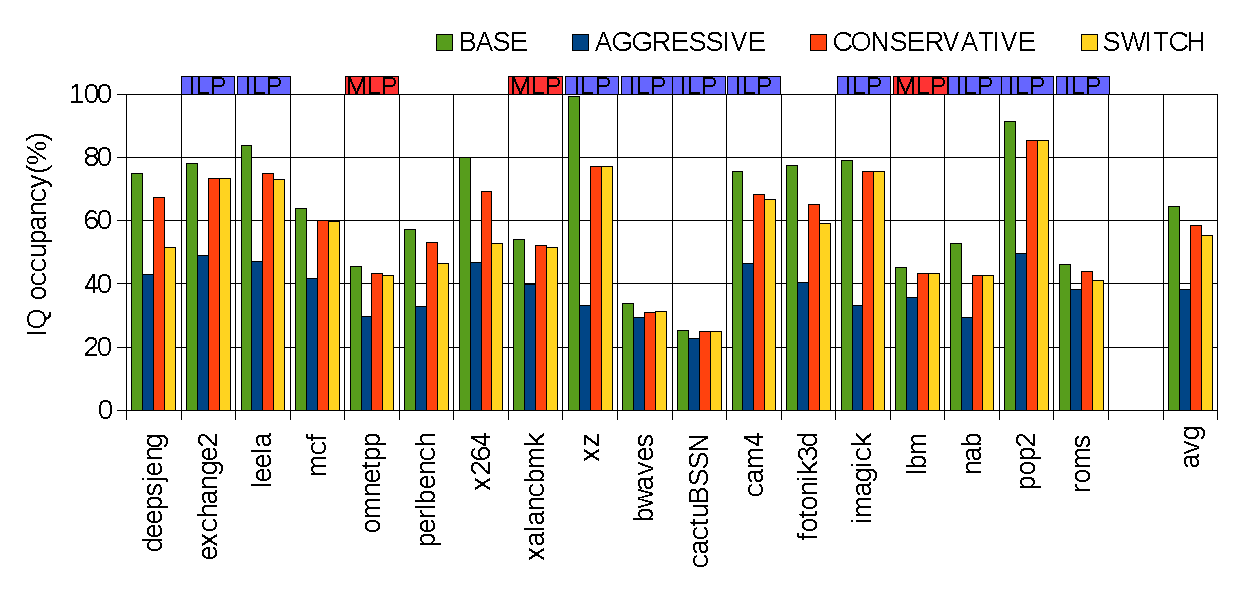
\includegraphics[keepaspectratio, scale=.8]{occupancy_16_1}
  \caption{IQ の占有率(16,1)}
  \label{fig:occupancy_16_1}
\end{figure}

\section{提案手法によるタグ比較回数削減と性能低下の評価}
\label{sec:eval_segIQ}
提案手法によるタグ比較回数の削減と性能低下に関して評価を行う.サブ・セグメントを使用せず,セグメント数は 16 とした.このセグメント数は,提案手法による性能低下とタグ比較回数のバランスを考慮し,提案手法の特徴をよく評価できるパラメータであると考え選んだものである.

なお,以降の評価において,(メイン・セグメント数,サブ・セグメント数) の形式でセグメント数を表記する.また,サブ・セグメントを使用しない場合は,サブ・セグメント数は 1 と表記する.今回の場合は(16,1)となる.

\subsection{タグ比較回数の削減}
\fig{comp_16_1}に,提案手法の BASE モデルに対するタグ比較回数の割合をベンチマークごとに示す.GM は全ベンチマークでの平均を表す.AGGRESSIVE と CONSERVATIVE のタグ比較回数削減に関しては,同図より,いずれのベンチマークにおいても,AGGRESSIVE のほうがタグ比較回数が少ないことがわかる.その差は 平均で 20\% 程度となっており,AGGRESSIVE モードのタグ比較回数を積極的に削減できるという性質が確認できる.

同図より SWITCH 方式では,平均で BASE モデルの 25\% 程度のタグ比較回数となっており,75\% の削減を達成している.

SWITCH 方式では,ILP や MLP の高いベンチマークにおいては CONSERVATIVE と同程度のタグ比較回数であるのに対して,そうでないベンチマークにおいては AGGRESSIVE に近いタグ比較回数となっていることがわかる.したがって,IQ の容量効率が重要でないベンチマークにおいては,AGGRESSIVE モードを選択して積極的にタグ比較回数の削減が行えていることがわかる.

\subsection{性能低下}
\fig{ipc_16_1}に,BASE に対する提案手法による性能低下をベンチマークごとに示す.同図より,SWITCH 方式による性能低下は最大で 3.5\% 程度であり,多くのベンチマークでは 0\% に近く性能はほとんど低下しないということが確認できる.

SWITCH 方式の有効性に関して述べる.同図より,ILP や MLP が高い xalancbmk や imagick,lbm などのベンチマークにおいて,AGGRESSIVE では大きく性能低下しているのに対して,CONSERVATIVE では性能低下が抑制されていることが分かる.そして SWITCH では,CONSERVATIVE と同程度の性能低下にとどまっている.従って,容量効率が性能にとって重要なプログラムにおいて,SWITCH 方式によって性能低下が抑制できていることが分かる.

\fig{occupancy_16_1}に各モデルでの IQ の占有率を示す.占有率とは,IQ の全エントリのうち使用されたエントリの割合であり,この値が BASE のそれに近いほど容量効率が低下していないことを示す.

同図より,AGGRESSIVE では BASE に対して占有率が大きく低下しているのに対して,CONSERVATIVE では占有率の低下がある程度抑制できていることが分かる.そして,ILP や MLP が高いベンチマークでは SWITCH 方式での占有率が CONSERVATIVE と同程度となっていることが分かる.このことからも,SWITCH 方式では,容量効率の性能に対する重要性に応じて適切にモードを選択し,容量効率の低下による性能低下を抑制できており,SWITCH 方式が有効であると言える.

\subsubsection{性能向上の原因}
\fig{ipc_16_1}より,いくつかのベンチマークでは性能が向上していることが分かる.この理由に関して説明する.一般にランダム・キュー方式の IQ には,命令がプログラム順に並んでいないため,最も優先して発行すべき命令の発行が遅れる可能性があるという欠点が存在する.ランダム・キューでは,命令の並びが年齢についてランダムになる一方,選択論理は,下のエントリほど優先して発行命令を選択するため,レディ命令が発行幅以上に存在する発行コンフリクトが生じた場合,誤った優先度で命令を選択することが生じる.

提案手法では IQ の容量効率が低下するため,IQ 内の命令数が少なくなり,結果的に発行コンフリクトが生じる確率が低下する.この結果,問題が生じにくくなり僅かに性能が向上する.

\fig{ipc_16_1}において,性能が向上するベンチマークの他に,ILP や MLP が高いにもかかわらず,AGGRESSIVE においても性能低下の小さいベンチマークがあることも分かる.こういったベンチマークにおいても,発行コンフリクトの緩和による性能向上が発生しているため,容量効率の低下による性能低下と中和されて,結果として性能低下が小さいと考えられる.

\begin{figure}[htb]
  \centering
  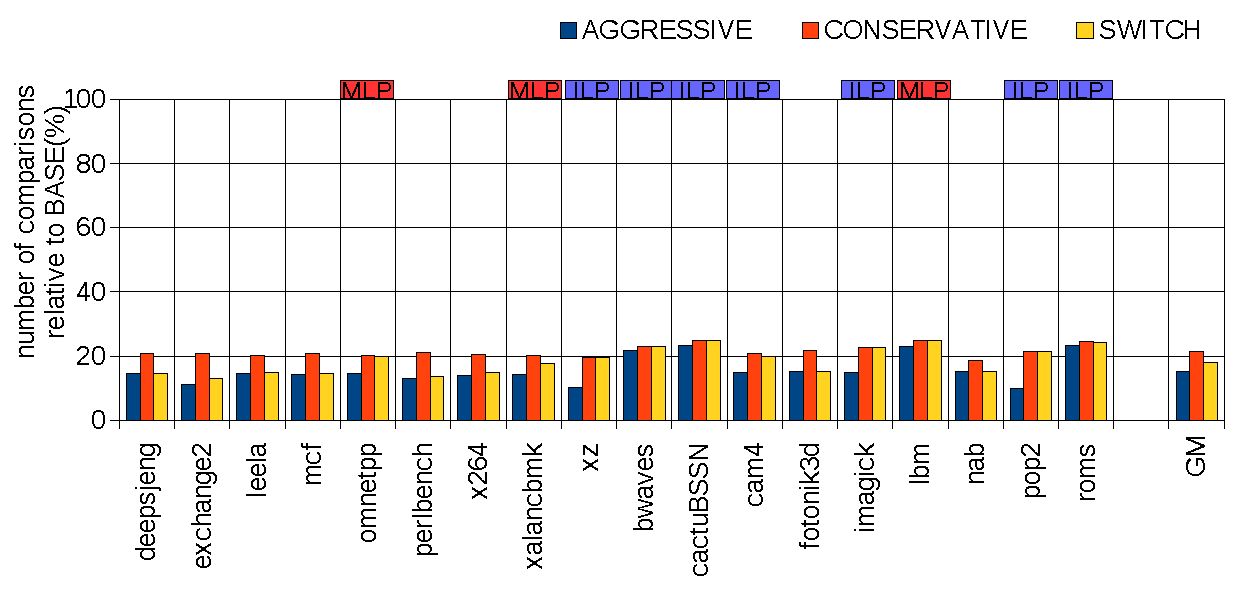
\includegraphics[keepaspectratio, scale=.8]{comp_8_2}
  \caption{提案手法によるタグ比較回数(8,2)}
  \label{fig:comp_8_2}
\end{figure}

\begin{figure}[htb]
  \centering
  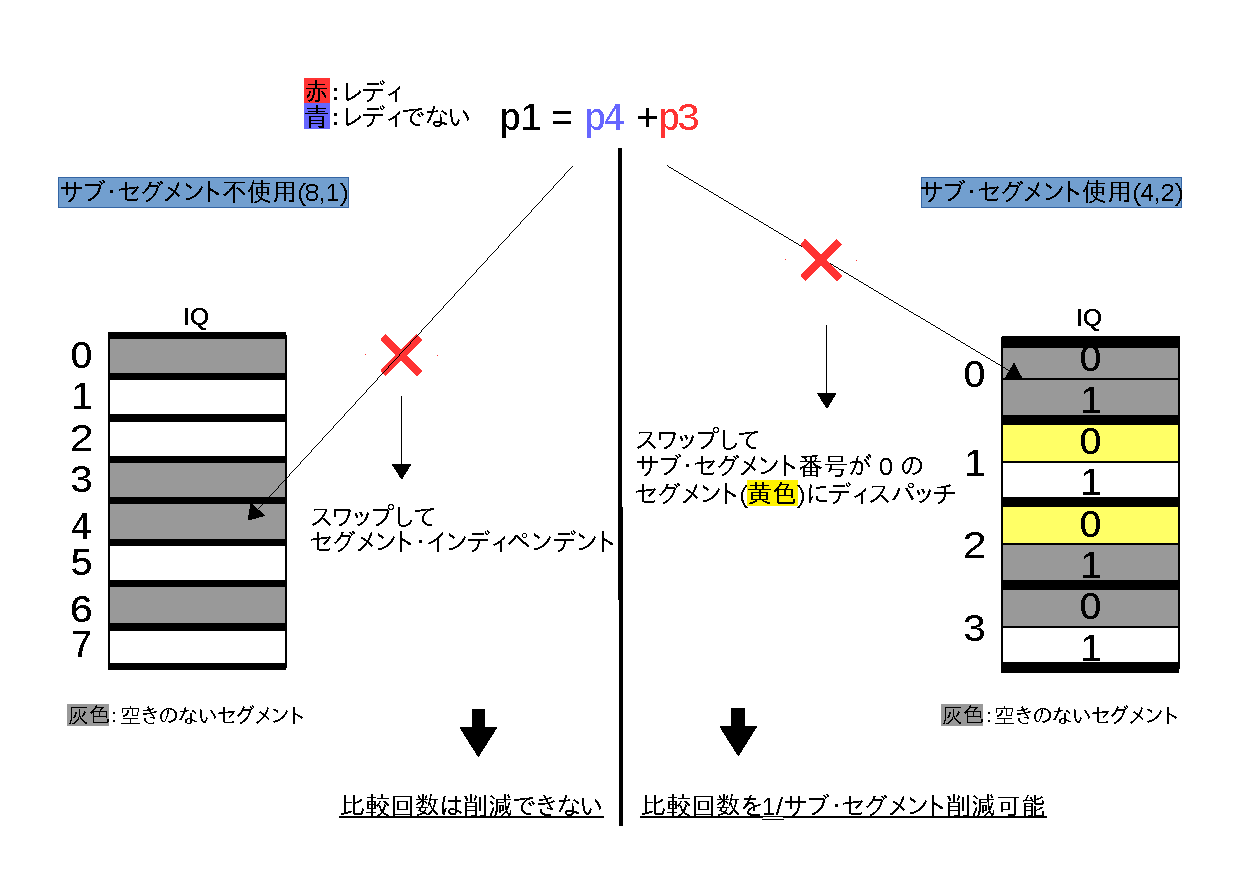
\includegraphics[keepaspectratio, scale=.8]{conservative_sub_seg}
  \caption{サブ・セグメントを使用する CONSERVATIVE モードにおけるタグ比較回数}
  \label{fig:conservative_sub_seg}
\end{figure}

\begin{figure}[htb]
  \centering
  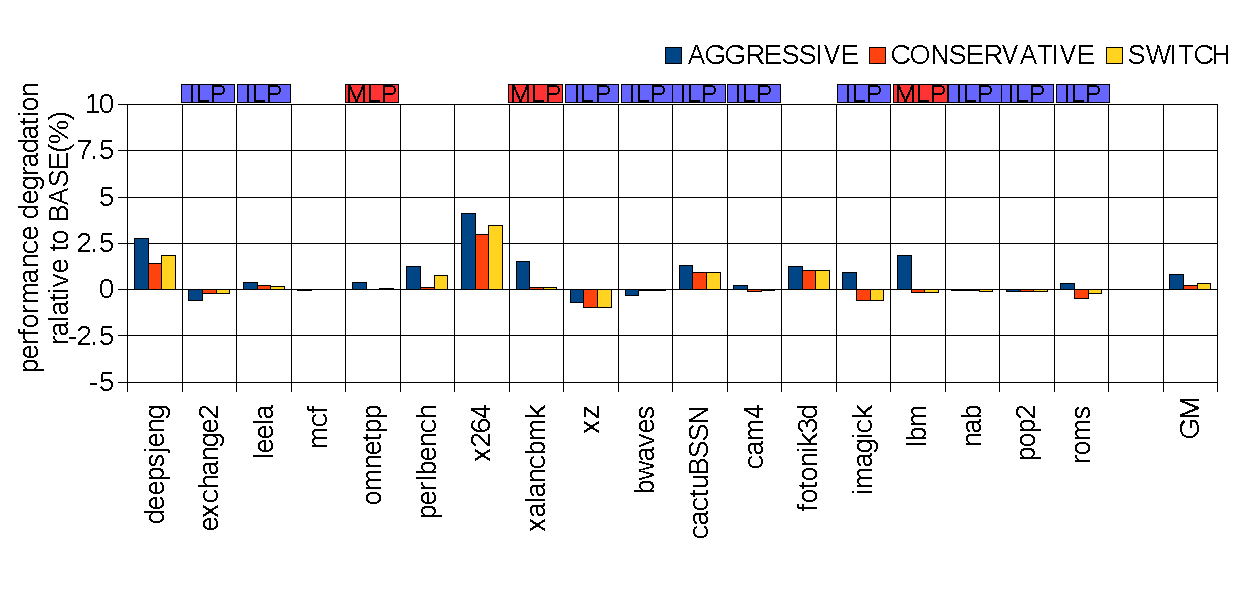
\includegraphics[keepaspectratio, scale=.8]{ipc_8_2}
  \caption{提案手法による性能低下(8,2)}
  \label{fig:ipc_8_2}
\end{figure}
\begin{figure}[htb]
  \centering
  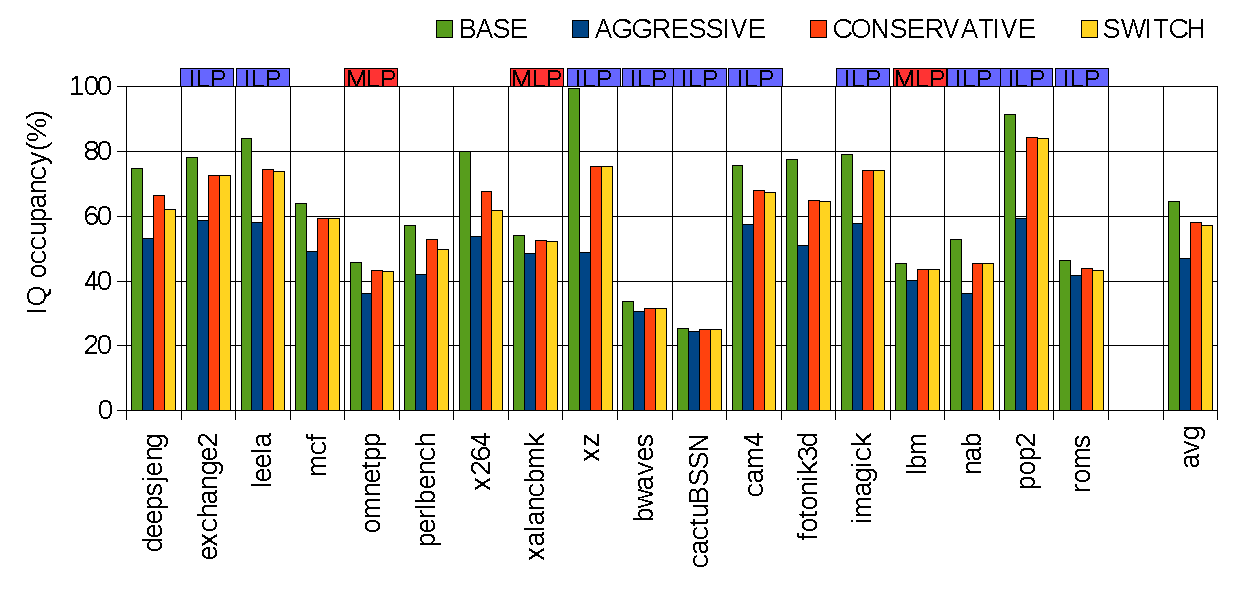
\includegraphics[keepaspectratio, scale=.8]{occupancy_8_2}
  \caption{IQ の占有率(8,2)}
  \label{fig:occupancy_8_2}
\end{figure}

\begin{table}[htb]
  \caption{(16,1)と(8,2)の比較}
  \footnotesize
  \center
    \begin{tabular}{cc|c|c|c} \hline \hline
     & & タグ比較回数 & 性能低下(最大) & 性能低下(平均)\\\hline
     & AGGRESSIVE  & 16\%  & 10.8\% & 0.6\% \\
    (16,1) & CONSERVATIVE & 35\% & 2.2\% & 0.3\% \\ \
     & SWITCH & 25\% & 3.8\% & -0.8\% \\ \hline
     & AGGRESSIVE & 15\% & 3.7\% & -0.1\% \\
    (8,2) & CONSERVATIVE & 21\% & 2.8\% & 0.3\% \\ 
     & SWITCH & 18\% & 3.4\% & -0.4\% \\ \hline
  \end{tabular}
  \label{tab:subseg_eval}
\end{table}

\section{サブ・セグメントに関する評価}
\label{sec:eval_subseg}
サブ・セグメントを使用する場合の提案手法に関して評価する.メイン・セグメント数が 8,サブ・セグメント数が 2 の場合((8,2)と表記する)に関して評価を行った.このセグメントの組み合わせは,(16,1) の場合とセグメントの総数が同じであり,比較の対象として適していると考え選んだものである.また,(8,2)の組み合わせは,\refsec{eval_ipc_comp}で説明するセグメントの分割数に関する評価において,最適と判断された組み合わせである.


\subsection{タグ比較回数の削減}
\fig{comp_8_2}に,提案手法の BASE モデルに対するタグ比較回数の割合をベンチマークごとに示す.また,\tab{subseg_eval}に,(16,1) と(8,2)の各評価モデルにおけるタグ比較回数の平均値,性能低下の最大値,性能低下の平均値を示す.

\tab{subseg_eval} より,(16,1)と (8,2)の CONSERVATIVE を比較すると,(16,1)の場合が平均で 35\% であるのに対して,(8,2) では 21 \% 程度と,(8,2)のほうがより削減できていることが分かる.これは,サブ・セグメントを使用する場合,\refsec{two_mode}で説明した CONSERVATIVE モードでのストールの回避を行った際にも,タグ比較の削減が可能となるためである.\fig{conservative_sub_seg}を用いて詳しく説明する.

図中に示す命令をディスパッチする場合を考える.サブ・セグメントを使用しない場合(図左側),第 1 ソース・タグ $p4$ によって決定されるセグメント(第 4 セグメント)に空きがなければ,CONSERVATIVE ではスワップを行い,セグメント・インディペンデントとしてディスパッチを行う.この場合,第 1 ソース・タグ $p4$ のタグ比較回数は削減されない.

一方で,サブ・セグメントを使用する場合(図右側),第 1 ソース・タグ$p4$によってメイン・セグメントが決定され,もし空きがなければ,スワップを行う.そして,第 1 ソース・タグ $p4$ によってサブ・セグメント番号が決定され,該当する番号のいずれかに空きがあれば(図中の黄色で示したセグメント),そのセグメントにディスパッチする.この場合,第 1 ソース・タグ $p4$ の比較は,タグの下位ビットがサブ・セグメント番号と一致する場合のみ行われるため,その比較回数は 「1 / サブ・セグメント数」まで削減が可能となる.

以上で説明したように,サブ・セグメントを用いると,CONSERVATIVE モードでストールの回避を行った際にも,タグ比較の削減が可能となる.その結果,CONSERVATIVE モードでの高いタグ比較削減率を達成することが出来る.

最後に SWITCH 方式に関して評価する.(16,1) の場合と同様に容量効率の重要性に応じてモードの切り替えができており,IQ の容量効率が重要でないベンチマークにおいては AGGRESSIVE モードと同程度の削減率を達成できている.

\subsection{性能低下}
\fig{ipc_8_2}に,BASE に対する提案手法による性能低下をベンチマークごとに示す.同図より,SWITCH 方式による性能低下は最大で 4\% 程度であり,多くのベンチマークでは 0\% に近く性能はほとんど低下しないということが確認できる.

AGGRESSIVE の性能低下率に関して考える.\tab{subseg_eval} より,(8,2) では,(16,1)と比較して AGGRESSIVE の性能低下率が低いことが分かる.これは,サブ・セグメントによって AGGRESSIVE モードでの容量効率の低下が抑制されているためであると考えられる.

\fig{occupancy_8_2} に,(8,2)の場合の IQ の占有率を示す.\fig{occupancy_16_1}と\fig{occupancy_8_2}の占有率を比較すると,(16,1)の場合は平均で 30\% 程度であった占有率が,(8,2)では平均で 40\% となっている.また,(16,1)の AGGRESSIVE において特に性能低下の大きかった imagick に関して見てみると,(16,1)の AGGRESSIVE では占有率が 35\% 程度で,性能低下が10\% であるのに対して,(8,2) の AGGRESSIVE では占有率が 65\% 近くまで上昇しており,その結果性能低下が 3\% 程度となっている.

以上の考察から,セグメントの総数が同じである場合,サブ・セグメントを使用することによって,AGGRESSIVE モードでの容量効率の低下による性能低下を抑制できることがわかった.

最後に,SWITCH 方式の有効性に関して説明する.(8,2)の場合,サブ・セグメントが有効であり,AGGRESSIVE での大幅な性能低下が見られないため,(16,1)の場合と比較して SWITCH 方式の有効性は高くないように見られる.しかし,imagick や lbm などのベンチマークにおいては AGGRESSIVE で発生する性能低下を抑制できている.CONSERVATIVE でのタグ比較削減率が高く,その結果 SWITCH 方式自体のタグ比較削減率も高くなっている.

\subsubsection{サブ・セグメントの評価のまとめ}
サブ・セグメントを使用すると,以下のメリットがあることがわかった.
\begin{itemize}
  \item CONSERVATIVE モードでのタグ比較回数がより削減できる
  \item AGGRESSIVE モードにおける性能低下が改善される
\end{itemize}
したがって,サブ・セグメントは有効な手法であると言える.

\section{SWITCH 方式のしきい値に関する評価}
\label{sec:eval_threshold}
SWITCH 方式において,ILP と ILP の高低を判定するために使用するしきい値に関する評価を行う.

\begin{figure}[htb]
  \centering
  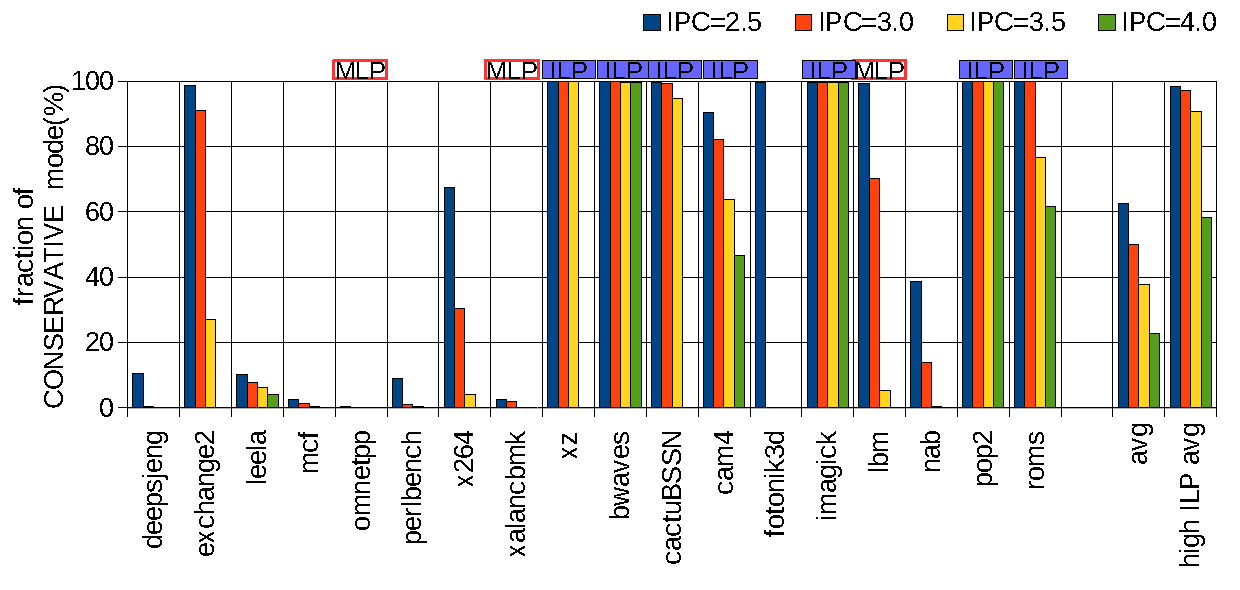
\includegraphics[keepaspectratio, scale=.8]{switch_IPC_rate}
  \caption{IPC を用いた SWITCH 方式の制御}
  \label{fig:switch_IPC_rate}
\end{figure}

\subsection{ILP の評価値}
ILP を評価する値として IPC と ISR の評価を行う.評価の方針としては,まず IPC と ISR のしきい値に関して適当な値を求める.適当ななしきい値は,しきい値を変化させた場合に,ILP の高いベンチマークにおいて CONSERVATIVE モードで実行される割合を評価することによって決定する.

その後,それぞれの評価値を利用する場合の提案手法によるタグ比較削減と性能低下を比較し,IPC と ISR のどちらがより適した評価指標か評価する.

\subsubsection{IPC による制御}
ILP の評価指標として,IPC を使用する場合の評価を行った.本評価は,セグメント数を(16,1)として行った.また,ILP による SWITCH 方式の制御のみ行い,MLP による制御は行っていない.

\fig{switch_IPC_rate}に,IPC のしきい値を変化させた場合の,CONSERVATIVE モードで実行される割合を示す.この割合が大きいほど,ILP が高いと判断され多くのサイクルが CONSERVATIVE モードで実行されていることを表す.また,各判例の IPC=X は,ILP が高いと判定する IPC のしきい値をX とした場合を示している.また,avg は全ベンチマークの平均を,high ILP avg は ILP の高いベンチマークでの平均を表している. 

当図より,IPC のしきい値が高くなるほど,CONSERVATIVE モードで実行される割合が小さくなっていることが分かる.これは,ILP が高いと判定される基準が厳しくなるためである.ILP の高いベンチマークに関して見ると,多くのベンチマークにおいて,しきい値が 3.5 の場合は CONSERVATIVE モードの割合が大きく,しきい値が 4.0 になると CONSERVATIVE モードの割合が小さくなっていることが分かる.high ILP avg を見ると,しきい値が 3.5 の場合は CONSERVATIVE モードの割合は 90\% 程度であるが,しきい値が 4.0 の場合は CONSERVATIVE モードの割合は 60\% 程度と小さくなる.

ILP が高い場合は CONSERVATIVE モードで実行することが望ましい.従って,IPC のしきい値は,3.5 程度が適当であるといえる.

\begin{figure}[htb]
  \centering
  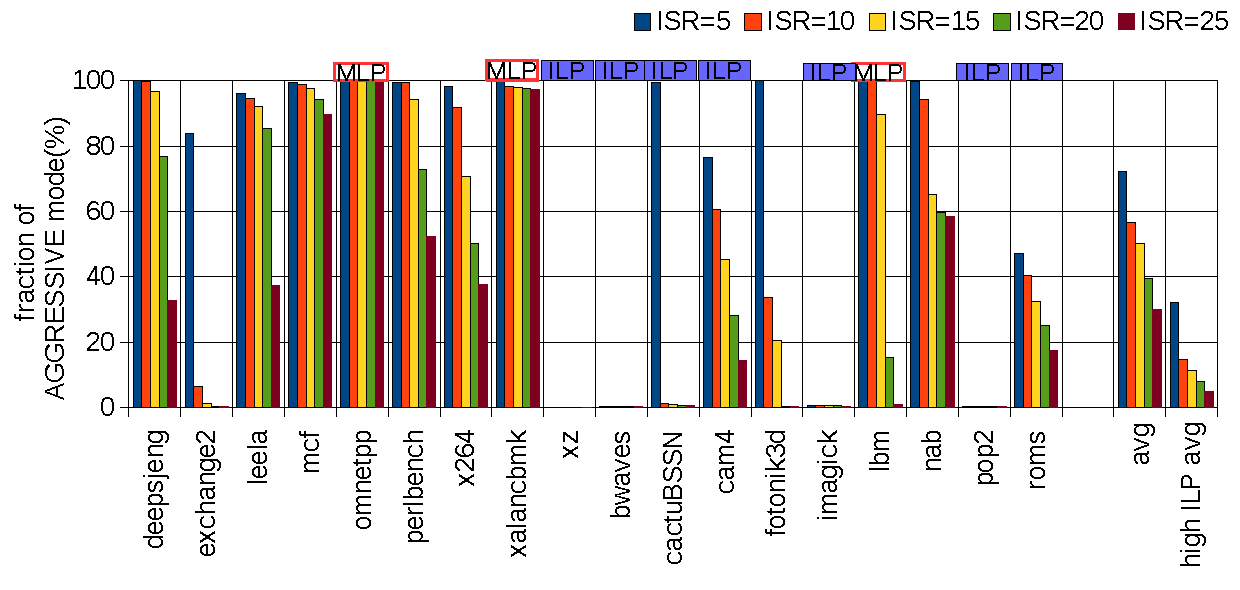
\includegraphics[keepaspectratio, scale=.8]{switch_ISR_rate}
  \caption{ISR を用いた SWITCH 方式の制御}
  \label{fig:switch_ISR_rate}
\end{figure}

\subsubsection{ISR による制御}
ILP の評価指標として,ISR を使用する場合の評価を行った.評価は IPC の場合と同様にセグメント数を(16,1)として行った.また,ILP による SWITCH 方式の制御のみ行い,MLP による制御は行っていない.

\fig{switch_ISR_rate}に,ISR のしきい値を変化させた場合の,CONSERVATIVE モードで実行される割合を示す.各判例の ISR=X は,ILP が高いと判定する ISR のしきい値を X とした場合を表す.

当図より,ISR のしきい値が低くなるほど,CONSERVATIVE モードで実行される割合が小さくなっていることが分かる.これは,ILP が高いと判定される基準が厳しくなるためである.high ILP avg を見ると,しきい値が 5 の場合は CONSERVATIVE モードの割合は 60\% 程度であるが,しきい値が 10 の場合は CONSERVATIVE モードの割合は 90\% 程度と大きくなる.

ILP が高い場合は CONSERVATIVE モードで実行することが望ましい.従って,ISR のしきい値は,10 程度が適当であるといえる.

\begin{figure}[htb]
  \centering
  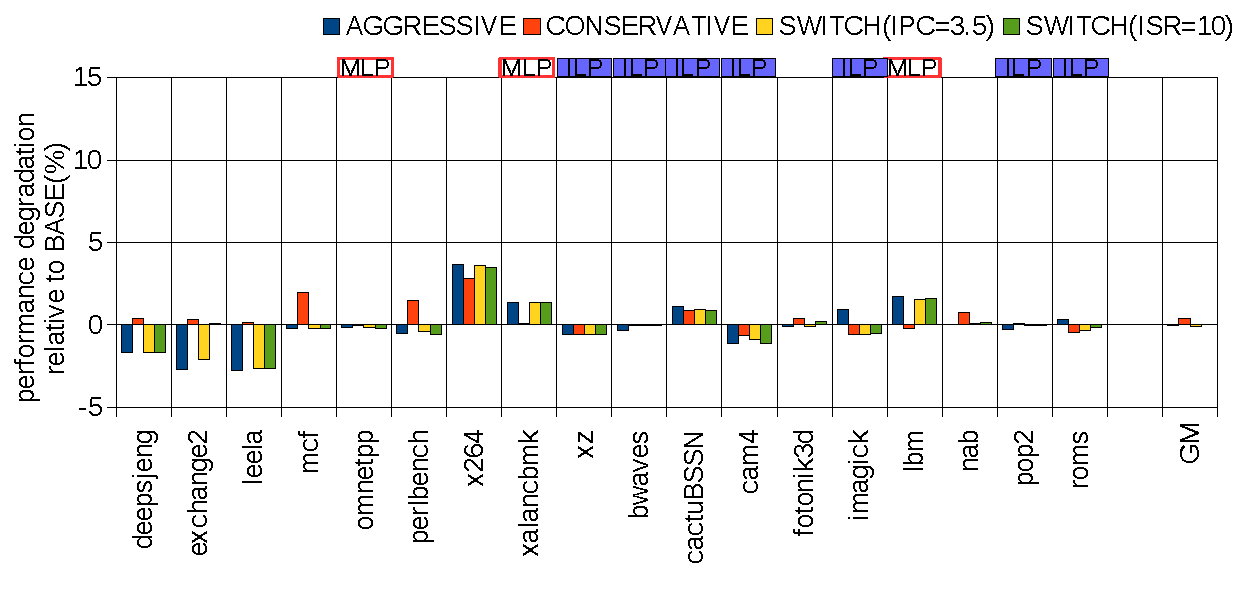
\includegraphics[keepaspectratio, scale=.8]{switch_ILP_performance}
  \caption{ILP による制御を行った SWITCH 方式による性能低下}
  \label{fig:switch_ILP_performance}
\end{figure}

\begin{figure}[htb]
  \centering
  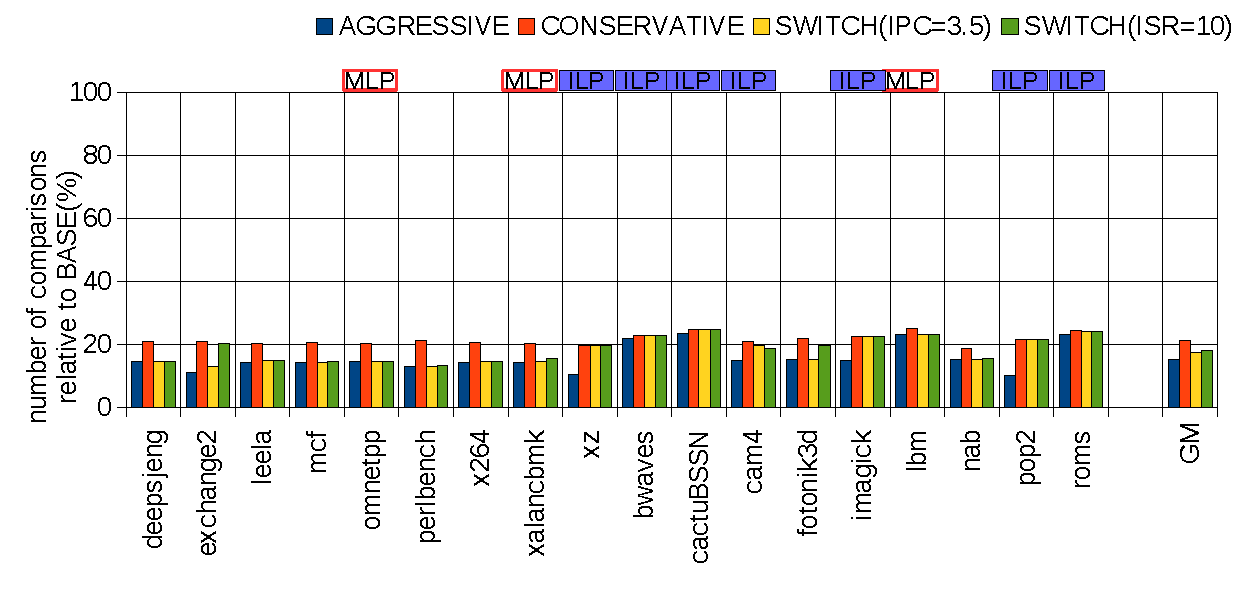
\includegraphics[keepaspectratio, scale=.8]{switch_ILP_comp}
  \caption{ILP による制御を行った SWITCH 方式によるタグ比較回数}
  \label{fig:switch_ILP_comp}
\end{figure}

\subsubsection{IPC と ISR の比較}
\fig{switch_ILP_performance}に,IPC と ISR を用いて制御を行う SWITCH 方式での性能低下を示す.MLP による制御は行っていない.同図より,ILP が高いベンチマークにおいては,IPC と ISR いずれの指標においても正しく評価できており,結果として SWITCH による性能低下が CONSERVATIVE と同程度に抑制できていることがわかる.また,ILP が高くないベンチマークにおいては,IPC と ISR による制御において大きな差はみられない.平均を見ても,IPC と ISR は同程度であると言える.

\fig{switch_ILP_comp}に,IPC と ISR を用いて制御を行う SWITCH 方式でのタグ比較回数を示す.タグ比較回数も,性能低下と同様に IPC と ISR で大きな差は見られないが,exchange2 と fotonik3d に関しては,IPC を用いた制御のほうが ISR を用いた制御よりもタグ比較回数が少ないことが分かる.この理由は,この 2 つベンチマークについては,IPC を用いた制御で ILP が低いと判定されているのに対して,ISR を用いた制御では ILP が高いと判定されているためである.

exchange2 及び fotonik3d は提案手法によって性能低下を起こさないベンチマークであるため,ILP が高いと判定されて CONSERVATIVE モードで実行されることは望ましくない.従って,これらのベンチマークを ILP が低いと判定できる IPC による制御のほうが適していると考えられる.

以上の評価から,ISR による制御は一部の ILP が低いベンチマークを ILP が高いと判定してしまうため,IPC を 用いた制御のほうがより適していると言える.SWITCH 方式における ILP の判定は,IPC を用いることとし,ILP が高いとする IPC のしきい値は 3.5 とする.

\subsection{MLPの評価値}
MLP を評価する値として LLC MPKI の評価を行う.評価の方針としては,LLC MPKI のしきい値に関して適当な値を求める.適当なしきい値は,しきい値を変化させた場合に,MLP の高いベンチマークにおいて,CONSERVATIVE モードで実行される割合を評価することによって決定する.

\begin{figure}[htb]
  \centering
  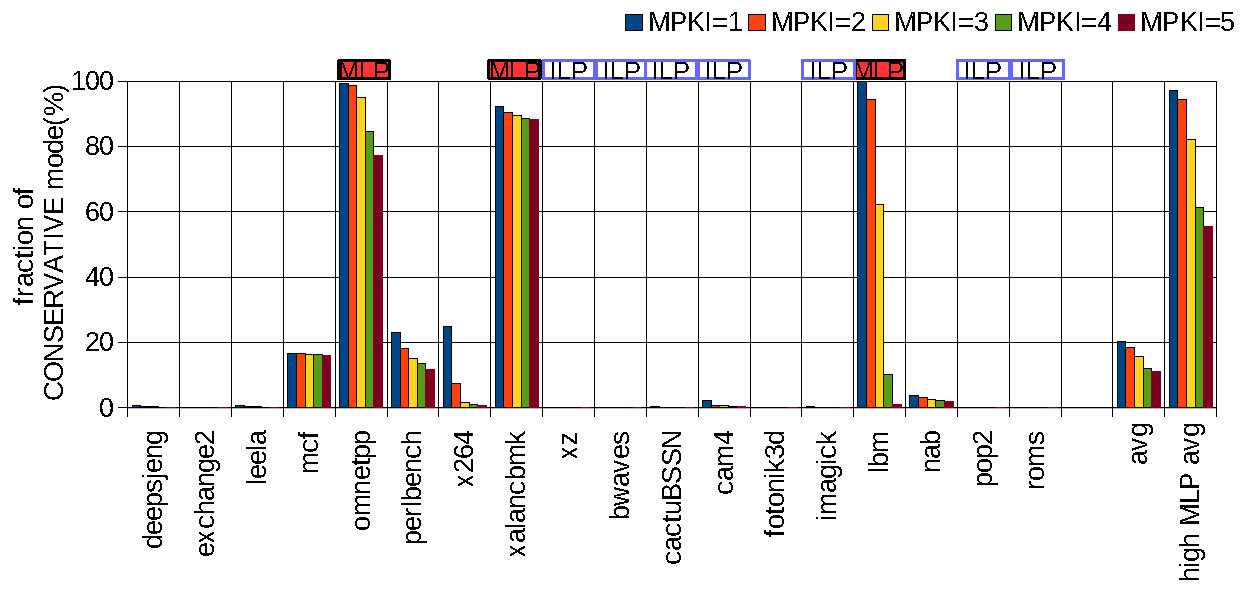
\includegraphics[keepaspectratio, scale=.8]{switch_MPKI_rate}
  \caption{LLC MPKI による SWITCH 方式の制御}
  \label{fig:switch_MPKI_rate}
\end{figure}

\subsubsection{LLC MPKI による制御}
本評価は,セグメント数を(16,1)として行った.また,MLP による SWITCH 方式の制御のみ行い,ILP による制御は行っていない.

\fig{switch_MPKI_rate}に,LLC MPKI のしきい値を変化させた場合の,CONSERVATIVE モードで実行される割合を示す.各判例の MPKI=X は,MLP が高いと判定する LLC MPKI のしきい値を X とした場合を表す.また,avg は全ベンチマークの平均を,high MLP avg は MLP の高いベンチマークでの平均を示している. 

当図より,LLC MPKI しきい値が高くなるほど,CONSERVATIVE で実行される割合が小さくなっていることが分かる.これは,LLC MPKI が高いと判定される基準が厳しくなるためである.

MLP の高いベンチマークに関して考える.omnetpp と lbm においては,しきい値が 2 以下場合は CONSERVATIVE モードの割合が大きいが,しきい値が 3 以上 になると CONSERVATIVE モードの割合が急激に小さくなっていることが分かる.xalancbmk に関しては,MLP の高いベンチマークの中でも特にメモリ・インテンシブなベンチマーク(LLC MPKI が 10 程度)であるため,しきい値を 5 まで増加させても CONSERVATIVE の割合は大きく変化しない.

MLP が高い場合は CONSERVATIVE モードで実行することが望ましい.従って,LLC MPKI のしきい値は,2 程度が適当であるといえる.

\begin{figure}[htb]
  \centering
  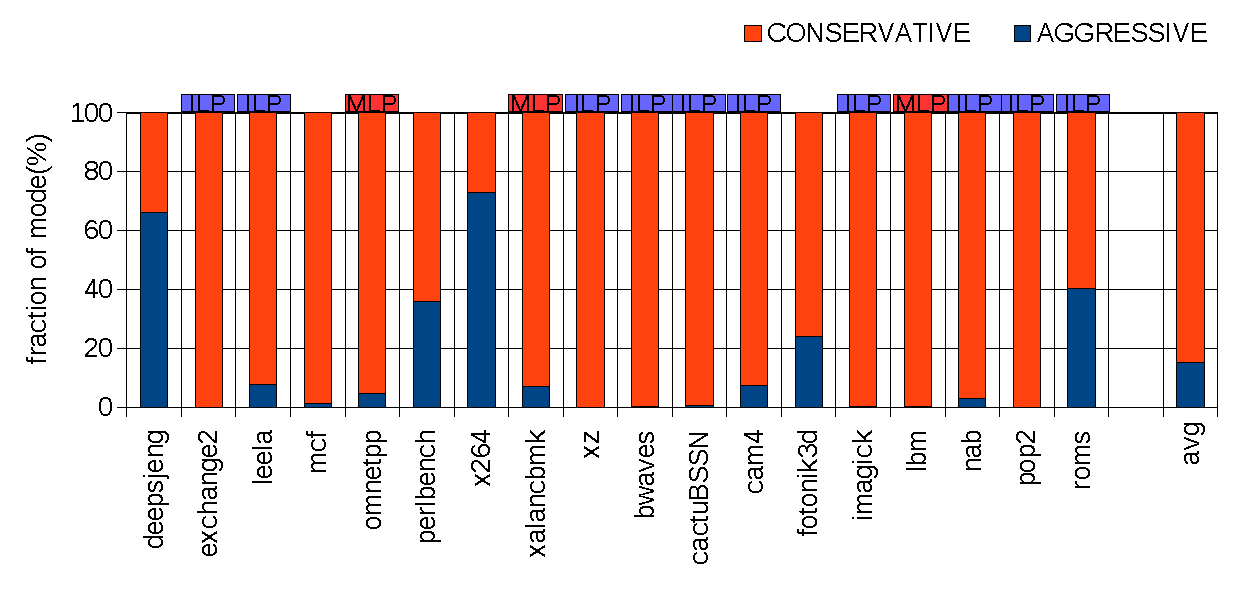
\includegraphics[keepaspectratio, scale=.8]{moderate_16_1}
  \caption{SWITCH 方式におけるモードの割合(16,1)}
  \label{fig:moderate_16_1}
\end{figure}

\begin{figure}[htb]
  \centering
  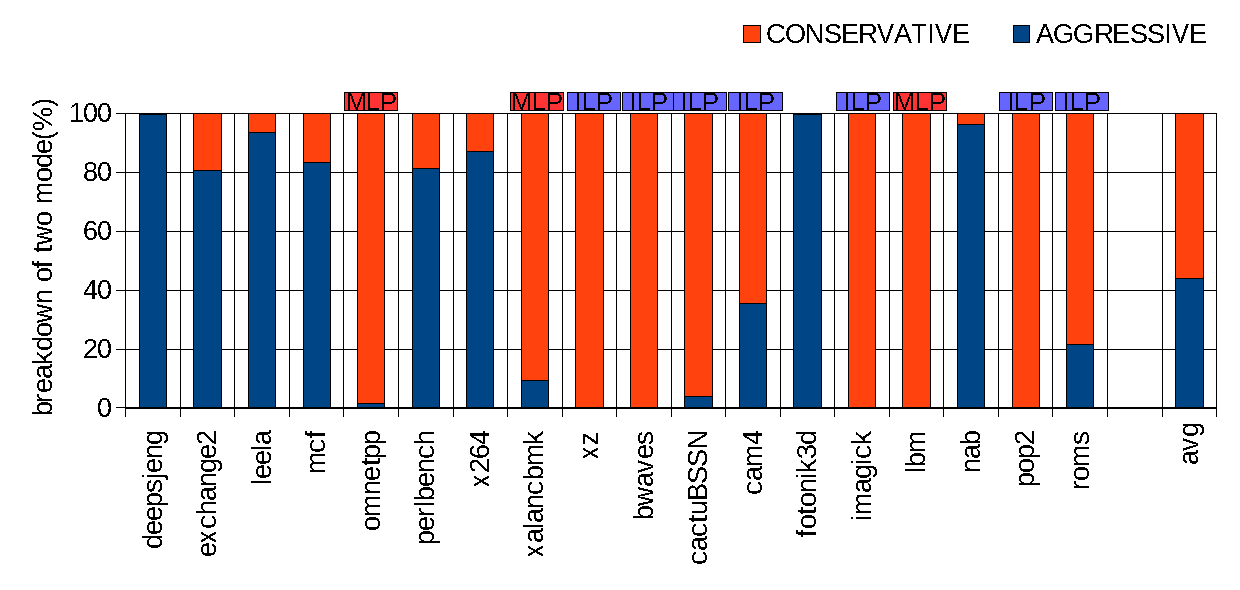
\includegraphics[keepaspectratio, scale=.8]{moderate_8_2}
  \caption{SWITCH 方式におけるモードの割合(8,2)}
  \label{fig:moderate_8_2}
\end{figure}

\subsection{IPC と LLC MPKI を用いた制御に関する評価}
ILP と MLP による制御を同時に行った場合に関して評価を行う.SWITCH 方式において,上記で決定したしきい値を用いて制御を行った際の,AGGRESSIVE モードと CONSERVATIVE モードで実行される割合を\fig{moderate_16_1}に示す.セグメント数は(16,1)である.

同図より,ILP 及び MLP の高いベンチマークは CONSERVATIVE モードの割合が多く,その他のベンチマークにおいては AGGRESSIVE モードの割合が高いことがわかる.したがって,容量効率の重要性に応じて適切なモードを選択できていると言える.

セグメント数が異なる場合でも同様の制御が行えるか確かめるため,(8,2)においても同様の測定を行った.結果を\fig{moderate_8_2}に示す.当図より (8,2) の場合においても,ILP または MLP が高いベンチマークは CONSERVATIVE モードの割合が高く,そうでないベンチマークでは AGGRESSIVE モードの割合が高いことがわかる.したがって,(16,1)で決定した IPC や LLC MPKI のしきい値は,異なるセグメント数であっても有効であるといえる.


\begin{figure}[htb]
  \centering
  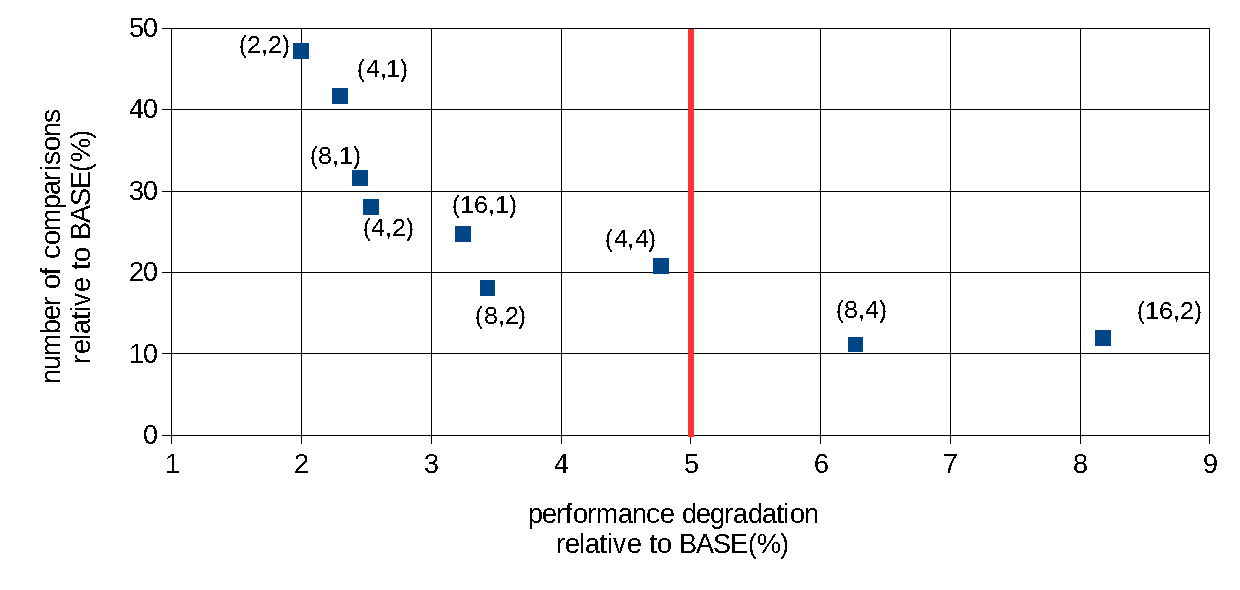
\includegraphics[keepaspectratio, scale=.8]{segment_num}
  \caption{セグメント数の違いによるタグ比較回数の削減と性能低下の散布図}
  \label{fig:segment_num}
\end{figure}

\section{セグメントの分割数に関する評価}
\label{sec:eval_ipc_comp}
セグメントの分割数を変化させて提案手法を評価し,最適であるセグメントの分割数を決定する.評価の基準としては,提案手法において次の条件を満たすセグメント数の組み合わせを最適と判断する.
\begin{itemize}
  \item 性能低下が全ベンチマークで 5\% 以下
  \item タグ比較回数の平均が最も少ない
\end{itemize}

\fig{segment_num}に,メイン・セグメント数とサブ・セグメント数を変化させた場合の,SWITCH 方式での性能低下とタグ比較回数の散布図を示す.図中の各点にはメイン・セグメント数とサブ・セグメント数を(メイン・セグメント数,サブ・セグメント数)という形式で付与している.横軸は最も性能低下が大きかったベンチマークにおける性能低下を示し,縦軸は全ベンチマークでの平均のタグ比較回数を示す.

同図より,セグメントの総数が増えると,タグ比較回数はより削減されるが,同時に性能低下も大きくなることがわかる.特に,(8,4)や(16,2)など,セグメントの総数が 32 を超えると,性能低下率が急激に増加している.

\fig{segment_num}において性能低下が 5\% より小さいセグメント数の組み合わせのうち,最もタグ比較回数の少ない(8,2)を最適が最適な組み合わせである.このときのタグ比較回数は 18\%(82\% 削減)となる.

また,サブ・セグメントを使用しない場合に最適な組み合わせは(16,1)であり,タグ比較回数は25\%(75\% 削減) となっている.

